\begin{figure*}[!t]
\centering
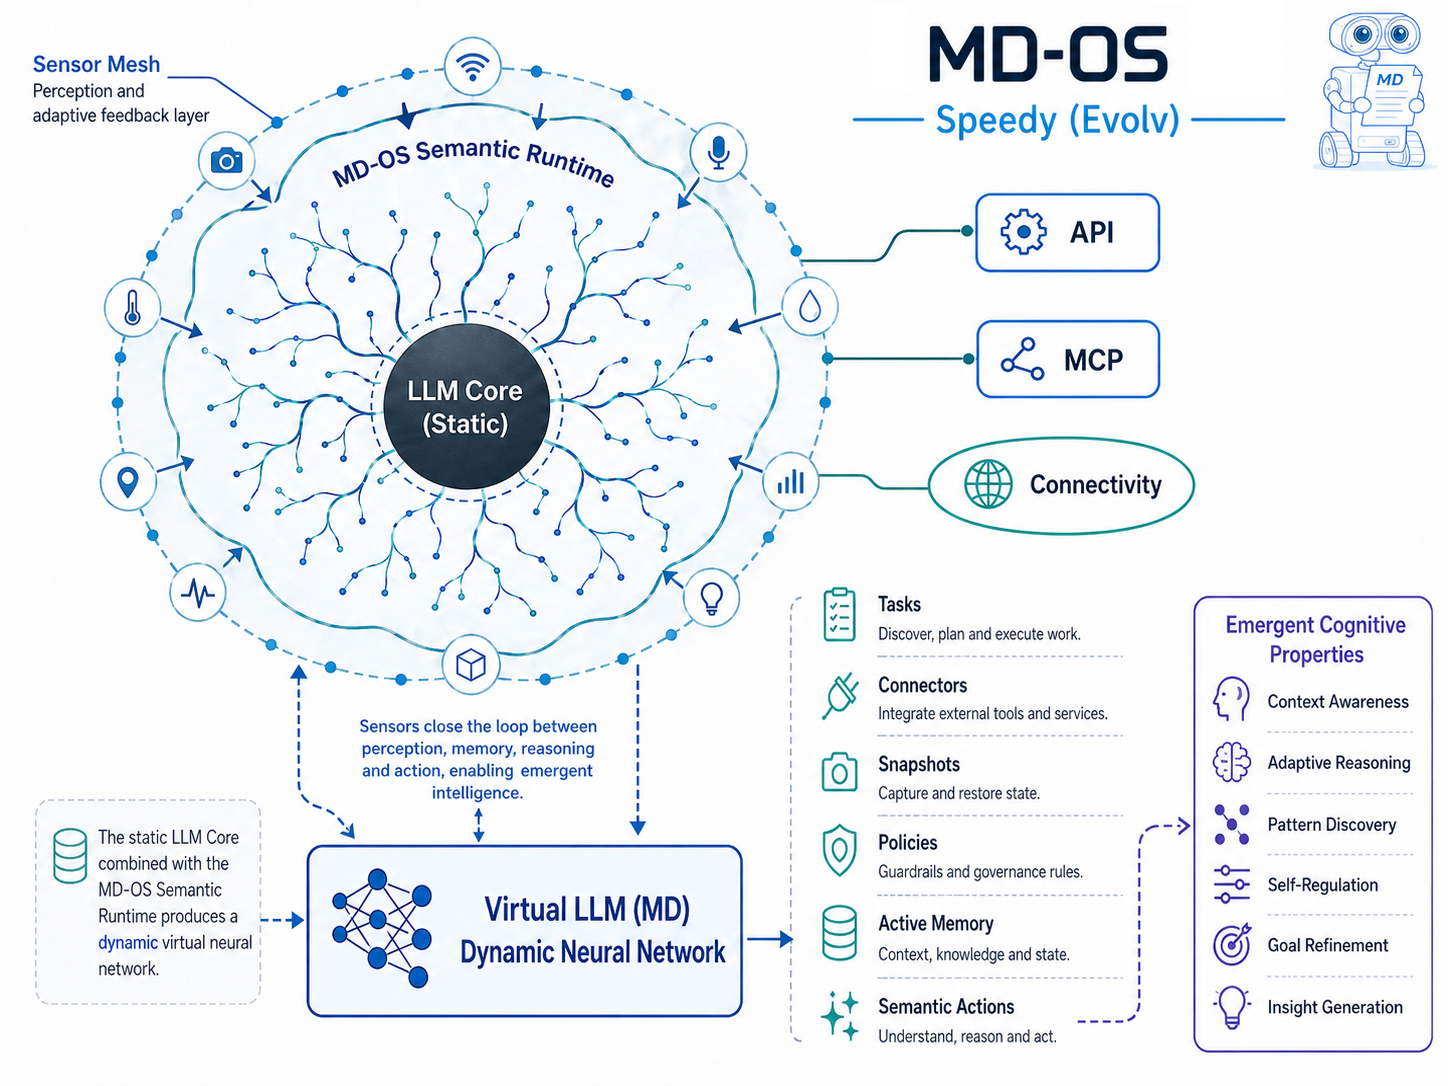
\includegraphics[width=0.96\textwidth]{figures/assets/md_os_cortex_proto_agi_schema.png}
\caption{\textbf{Original MD-OS CORTEX proto-AGI conceptual schema.}
The diagram states the central idea directly: a comparatively stable LLM core
is surrounded by the APFC, a dynamic semantic and operational network that closes the
loop among sensors, active memory, tasks, policies, connectors, external
systems, and actions.  Its persistent representation is the Artificial
Prefrontal Cortex Graph (APFCG), visible and navigable in Obsidian through its
linked Markdown nodes.  In the v5 formulation, the ``Virtual LLM (MD) Dynamic
Neural Network'' is interpreted as APFCG external to the model, not as an
unverified claim of a literal neural network.  APFCG becomes a candidate for
parametric consolidation only through the separately gated graph-to-weights
process.  The diagram is a
conceptual architecture, not evidence that Markdown files are biological
neurons or that model weights are already being updated.}
\label{fig:original-cortex-schema}
\end{figure*}
